\documentclass[12pt]{article}
\usepackage[margin=1.5cm]{geometry}
\usepackage{parskip}
\usepackage{amsmath}
\usepackage{amssymb}
\usepackage{amsfonts}
\usepackage{enumitem}
\usepackage{graphicx}
\usepackage{stmaryrd}
\graphicspath{ {./images/} }


\begin{document}
\begin{enumerate}[label=(\alph*)]
  \item
    The idea behind fibbing is to inject paths by adding virtual nodes and links that will always constitute a shortest path, and arrange these in a way to force a particular real path around the network.

    For example, in the diagram below, we show how fibbing would augment the network.

    At node $B$, we inject false link-state information that is as if $C$ has a better path to $D2$ by going via virtual node $V_1$, which is along the link between $A$ and $C$. In reality, this virtual node does not exist, so traffic sent to it will instead just reach $A$, at which point $A$ will forward it to $B$, then $X$, to reach $D_2$. The reason this is allowed to work is the flooding nature of link-state protocols, so by injecting information at just one point, it floods throughout the network and we are able to reach a steady state.

    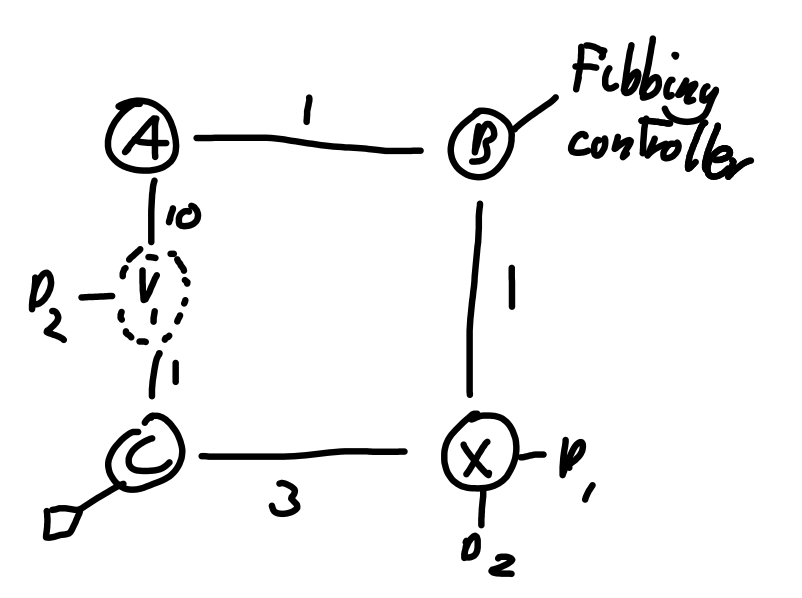
\includegraphics[scale=0.4]{fibbing}

    In order to determine what information to inject, we might start by inserting virtual nodes between $AB$ and $BX$ as well, in order to ensure that they always send data along the correct paths, but when injecting into the network we can merge these nodes and still get the same behaviour (like we have done here).

  \item

    The basic idea behind this algorithm is when a direct link from node $A$ to node $B$ is saturated, i.e. cannot hold any more capacity, then we need to choose a tandem node $C$ such that data flows along $ACB$ instead.

    The algorithm is incredibly simple. We simply pick a random node $C$ as our tandem, and keep using it as our tandem until it fails. This requires no analysis of traffic or centralized control, so has very low control overhead.

    The idea behind why this works is that at large scale, this essentially uniformly load balances in its nature.

    We might also choose to implement trunk reservation, where we only allow a fraction of the traffic for a tandem to be used for this load balancing, and the rest for its own direct links, ensuring that we can still (somewhat) guarantee service to other nodes connected to our tandem.

    There are alternatives, such as choosing 3-hop paths instead, but these tend not to have much benefit. 


        
\end{enumerate}
\end{document}
